% ============================================================================
%  SECCIÓN 2.6: WIREFRAMES INICIALES
% ============================================================================

\section{Wireframes iniciales}

Los wireframes son representaciones esquem\'aticas de baja fidelidad de las
pantallas de una aplicaci\'on, que permiten validar la estructura y la
ubicaci\'on de los elementos antes de la implementaci\'on \citep{pressman2010,
nielsen1994}. De acuerdo con la gu\'ia del avance, se presentan los wireframes
iniciales de las pantallas m\'inimas requeridas: bienvenida (splash), inicio de
sesi\'on, registro, pantalla principal y detalle de un escenario.

\subsection{Pantalla de bienvenida (Splash)}

Muestra el logotipo y el nombre provisional de la aplicaci\'on, junto con un
bot\'on que da inicio al recorrido de la aplicaci\'on.

\subsection{Pantalla de inicio de sesi\'on}

Permite al usuario ingresar su correo electr\'onico y contrase\~na, con un bot\'on
para iniciar sesi\'on y un enlace hacia el registro de nuevos usuarios.

\subsection{Pantalla de registro}

Recoge los datos b\'asicos del usuario (nombre, correo electr\'onico y
contrase\~na) y permite crear la cuenta.

\subsection{Pantalla principal (mapa)}

Es la pantalla central de la aplicaci\'on: incluye la barra de b\'usqueda, el
mapa interactivo con la ubicaci\'on de los escenarios y la navegaci\'on
principal (inicio, b\'usqueda y perfil).

\subsection{Pantalla de detalle de un escenario}

Muestra la ficha del escenario: fotograf\'ia, nombre, disciplinas, horarios y
un bot\'on para guardarlo como favorito.

\begin{figure}[H]
  \centering
  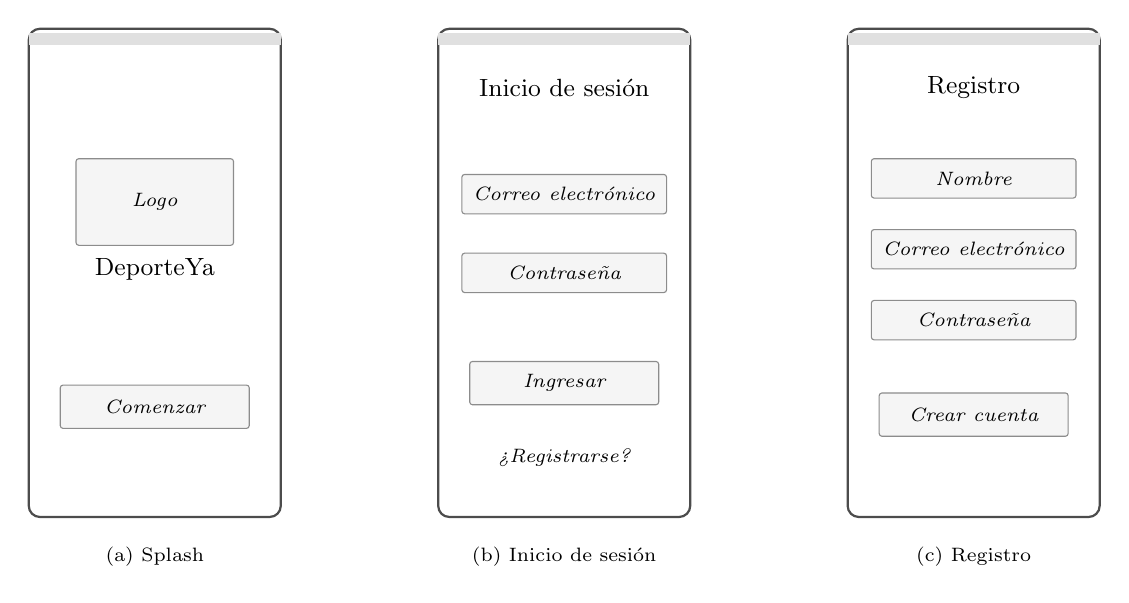
\begin{tikzpicture}[
      tel/.style={draw=black!70, thick, rounded corners=4pt, minimum width=3.2cm, minimum height=6.2cm},
      zona/.style={draw=black!45, thin, rounded corners=1pt, fill=gray!8},
      etiqueta/.style={font=\scriptsize\itshape, align=center},
      etqPantalla/.style={font=\scriptsize, align=center}
    ]
    % --- (a) Splash ---
    \begin{scope}[xshift=0cm]
      \node[tel] (a1) at (0,0) {};
      \fill[black!12] (-1.6,2.9) rectangle (1.6,3.05);
      \node[zona, minimum width=2.0cm, minimum height=1.1cm] at (0,0.9) {};
      \node[etiqueta] at (0,0.9) {Logo};
      \node[font=\small] at (0,0.05) {DeporteYa};
      \node[zona, minimum width=2.4cm, minimum height=0.55cm] at (0,-1.7) {};
      \node[etiqueta] at (0,-1.7) {Comenzar};
      \node[etqPantalla] at (0,-3.6) {(a) Splash};
    \end{scope}

    % --- (b) Inicio de sesión ---
    \begin{scope}[xshift=5.2cm]
      \node[tel] (b1) at (0,0) {};
      \fill[black!12] (-1.6,2.9) rectangle (1.6,3.05);
      \node[font=\small] at (0,2.35) {Inicio de sesi\'on};
      \node[zona, minimum width=2.6cm, minimum height=0.5cm] at (0,1.0) {};
      \node[etiqueta] at (0,1.0) {Correo electr\'onico};
      \node[zona, minimum width=2.6cm, minimum height=0.5cm] at (0,0.0) {};
      \node[etiqueta] at (0,0.0) {Contrase\~na};
      \node[zona, minimum width=2.4cm, minimum height=0.55cm] at (0,-1.4) {};
      \node[etiqueta] at (0,-1.4) {Ingresar};
      \node[etiqueta] at (0,-2.35) {¿Registrarse?};
      \node[etqPantalla] at (0,-3.6) {(b) Inicio de sesi\'on};
    \end{scope}

    % --- (c) Registro ---
    \begin{scope}[xshift=10.4cm]
      \node[tel] (c1) at (0,0) {};
      \fill[black!12] (-1.6,2.9) rectangle (1.6,3.05);
      \node[font=\small] at (0,2.35) {Registro};
      \node[zona, minimum width=2.6cm, minimum height=0.5cm] at (0,1.2) {};
      \node[etiqueta] at (0,1.2) {Nombre};
      \node[zona, minimum width=2.6cm, minimum height=0.5cm] at (0,0.3) {};
      \node[etiqueta] at (0,0.3) {Correo electr\'onico};
      \node[zona, minimum width=2.6cm, minimum height=0.5cm] at (0,-0.6) {};
      \node[etiqueta] at (0,-0.6) {Contrase\~na};
      \node[zona, minimum width=2.4cm, minimum height=0.55cm] at (0,-1.8) {};
      \node[etiqueta] at (0,-1.8) {Crear cuenta};
      \node[etqPantalla] at (0,-3.6) {(c) Registro};
    \end{scope}
  \end{tikzpicture}
  \caption{Wireframes de baja fidelidad de las pantallas de acceso}
\end{figure}

\begin{figure}[H]
  \centering
  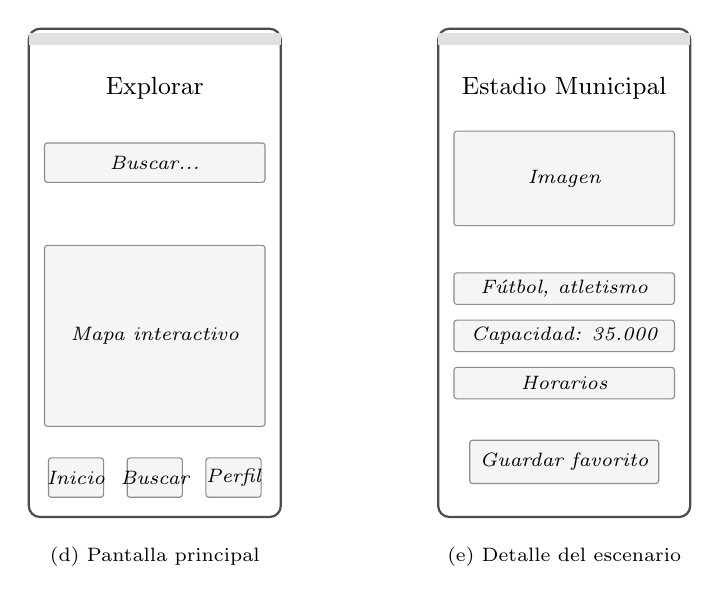
\begin{tikzpicture}[
      tel/.style={draw=black!70, thick, rounded corners=4pt, minimum width=3.2cm, minimum height=6.2cm},
      zona/.style={draw=black!45, thin, rounded corners=1pt, fill=gray!8},
      etiqueta/.style={font=\scriptsize\itshape, align=center},
      etqPantalla/.style={font=\scriptsize, align=center}
    ]
    % --- (d) Pantalla principal (mapa) ---
    \begin{scope}[xshift=0cm]
      \node[tel] (d1) at (0,0) {};
      \fill[black!12] (-1.6,2.9) rectangle (1.6,3.05);
      \node[font=\small] at (0,2.35) {Explorar};
      \node[zona, minimum width=2.8cm, minimum height=0.5cm] at (0,1.4) {};
      \node[etiqueta] at (0,1.4) {Buscar...};
      \node[zona, minimum width=2.8cm, minimum height=2.3cm] at (0,-0.8) {};
      \node[etiqueta] at (0,-0.8) {Mapa interactivo};
      \node[zona, minimum width=0.7cm, minimum height=0.5cm] at (-1.0,-2.6) {};
      \node[etiqueta] at (-1.0,-2.6) {Inicio};
      \node[zona, minimum width=0.7cm, minimum height=0.5cm] at (0,-2.6) {};
      \node[etiqueta] at (0,-2.6) {Buscar};
      \node[zona, minimum width=0.7cm, minimum height=0.5cm] at (1.0,-2.6) {};
      \node[etiqueta] at (1.0,-2.6) {Perfil};
      \node[etqPantalla] at (0,-3.6) {(d) Pantalla principal};
    \end{scope}

    % --- (e) Detalle del escenario ---
    \begin{scope}[xshift=5.2cm]
      \node[tel] (e1) at (0,0) {};
      \fill[black!12] (-1.6,2.9) rectangle (1.6,3.05);
      \node[font=\small] at (0,2.35) {Estadio Municipal};
      \node[zona, minimum width=2.8cm, minimum height=1.2cm] at (0,1.2) {};
      \node[etiqueta] at (0,1.2) {Imagen};
      \node[zona, minimum width=2.8cm, minimum height=0.4cm] at (0,-0.2) {};
      \node[etiqueta] at (0,-0.2) {F\'utbol, atletismo};
      \node[zona, minimum width=2.8cm, minimum height=0.4cm] at (0,-0.8) {};
      \node[etiqueta] at (0,-0.8) {Capacidad: 35.000};
      \node[zona, minimum width=2.8cm, minimum height=0.4cm] at (0,-1.4) {};
      \node[etiqueta] at (0,-1.4) {Horarios};
      \node[zona, minimum width=2.4cm, minimum height=0.55cm] at (0,-2.4) {};
      \node[etiqueta] at (0,-2.4) {Guardar favorito};
      \node[etqPantalla] at (0,-3.6) {(e) Detalle del escenario};
    \end{scope}
  \end{tikzpicture}
  \caption{Wireframes de baja fidelidad de las pantallas principales}
\end{figure}
